%%%% ijcai09.tex

\typeout{IJCAI-09 Instructions for Authors}

% These are the instructions for authors for IJCAI-09.
% They are the same as the ones for IJCAI-07 with superficical wording
%   changes only.

\documentclass{article}
% The file ijcai09.sty is the style file for IJCAI-09 (same as ijcai07.sty).
\usepackage{ijcai09}
\usepackage{booktabs}

% Use the postscript times font!
\usepackage{times}
\usepackage{amsmath}
\usepackage{graphicx}
\usepackage{tabularx}

% the following package is optional:
%\usepackage{latexsym} 

% Following comment is from ijcai97-submit.tex:
% The preparation of these files was supported by Schlumberger Palo Alto
% Research, AT\&T Bell Laboratories, and Morgan Kaufmann Publishers.
% Shirley Jowell, of Morgan Kaufmann Publishers, and Peter F.
% Patel-Schneider, of AT\&T Bell Laboratories collaborated on their
% preparation.

% These instructions can be modified and used in other conferences as long
% as credit to the authors and supporting agencies is retained, this notice
% is not changed, and further modification or reuse is not restricted.
% Neither Shirley Jowell nor Peter F. Patel-Schneider can be listed as
% contacts for providing assistance without their prior permission.

% To use for other conferences, change references to files and the
% conference appropriate and use other authors, contacts, publishers, and
% organizations.
% Also change the deadline and address for returning papers and the length and
% page charge instructions.
% Put where the files are available in the appropriate places.

\title{Employing Machine Learning for Fraudulence Detection across Credit Card Transactions}
\author{Nick Austin, Wes Bovee, Brayden Christensen, Cole Edgren, Spencer Jorgensen\\
CS 201R, Winter 2024\\
Department of Computer Science\\
Brigham Young University \\}

\begin{document}

\maketitle

\begin{abstract}
Recent efforts to combat the ongoing surge in financial fraud have included the harnessment of machine learning techniques to construct anomaly detection models for various forms of payment.
In this paper, we analyze the utility of machine learning algorithms in classifying the legitimacy of credit card transactions. Data was collected from Kaggle.com and subsequently preprocessed for training.
We selected features from the original dataset and engineered new features to incorporate more relevant variables into the data. Novel machine learning models, including Decision Tree, Logistic Regression, and XGBoost 
were implemented, trained, and evaluated against an alloted test portion of the final prepared dataset on their ability to correctly mark a credit card transaction as legitimate or fraudulent. Initial results demonstrated excellent performance 
(\(> \text{99\% classification accuracy}\)) with tree-based models. The high capability of these models in detecting anomalies across hundreds of thousands of transactions emphasizes the potential of machine learning for effective fraud prevention.
\end{abstract}

\section{Introduction}
Financial fraud is an evolving identity crime that affects millions worldwide annually.
In particular, the advent of convenient and accessible electronic payment systems such as those linked through mobile devices,
personal accounts, or software applications carries a heightened risk for financial security breaches. These emerging technologies combined with the substantial amount of transactions performed each day warrants a need for autonomous monitoring that extends beyond the practical scope of human capability. With modern advancements in data science, automatic early threat detection poses as a solution to mitigating the consequences of compromised financial information. Corporations have recently begun to implement early alert systems by training anomaly detection machine learning models on payment transaction data. Depending on the type of transaction, certain indicators may be important predictors in flagging a fraudelent payment, such as the amount of money transacted, the time of the transaction, or whether or not a card chip was used to complete the payment. 

As with many machine learning experiments, data quality, characterisitics, and amount is paramount to capturing the subtle patterns and relationships necessary to make accurate predictions. Unfortunately, in our search for appropriate data, we were faced with limitations from publicly available datasets due to customer privacy concerns. Despite this bottleneck, we postulated that general trends for financial fraud could still be replicated within available datasets and help formulate valuable and interpretable insights from prediction results. Throughout this paper, we collect and prepare transaction data, implement a variety of machine learning models, and examine classification ability through multiple metric assessments. 



\section{Methods}

\subsection{Data Collection}
Due to the confidential nature of consumer financial information, directly obtaining nonsynthetic data of adequate quality and scope proved difficult; in fact, we found that acquiring such data with interpretable features would not be possible with current legal restrictions. Eventually, we were able to locate two datasets from Kaggle.com, one which was synthteic, and the other containing geniune anonymized credit card transactions.  Both datasets contained labeled instances that were marked as fraudelent by a binary value of 1 and 0 otherwise. 

\subsection{Dataset 1}
The initial dataset, which we will refer to as Dataset 1, contained precisely 1,000,000 unique transactions characterized by several features as outlined in Table 1. Continuous features were standardized using standard score. Upon further inspection of the dataset, an immediate concern arose from the highly imbalanced class distribution: less than 1/10 instances were classified as fraudelent, while the majority of the other instances were legitimate. Prior to addressing the class distribution of the data, we decided to retain a copy of this imbalanced data for experimentation with machine learning models suited for anomaly detection to gather preliminary insights.

 In addition to the original imbalanced data for the anomaly detection models, we further prepared balanced data for more general use algorithms. In an effort to combat potential bias that could favor patterns across the legitimate transactions, we oversampled the minority fraudelent class using ADASYN (Adaptive Synthetic Sampling). Our choice of ADASYN instead of convential SMOTE (Synthetic Minority Oversampling) is based on ADASYN's  algorithmic design of generating synthetic minority samples through K-Nearest Neighbors that are closer to the majority samples and ultimately more difficult to learn. By this approach, we hypothesized subtle relationships in the minority class had a better chance of being captured by our models. 

\begin{table}[h]
\centering
\begin{tabular}{ll} 
\toprule
Feature & Data Type \\
\midrule
distance\_from\_home & continuous \\
distance\_from\_last\_transaction & continuous \\
ratio\_to\_median\_purchase\_price & continuous \\
repeat\_retailer & boolean \\
used\_chip & boolean \\
used\_pin\_number & boolean \\
online\_order & boolean \\
\bottomrule
\end{tabular}
\caption{Dataset 1 Features} % Caption for the table
\label{tab:dataset_features}
\end{table}

\subsection{Dataset 2}
In an effort to diversify our findings, we also trained models on a dataset that contains anonymized credit card transactions of European cardholders from 2013, which we will refer to as Dataset 2. It is the only publicly available dataset of our knowledge that contains actual, nonsynthetic transaction instances. As mentioned previously, customer privacy regulations necessitate a need for anonymity. Following this, the data was normalized and transformed by performing Principal Component Analysis to the original raw data, creating principal components V1-V28, which are the accompanied by only the following features: \texttt{Time}: time since transaction in seconds, \texttt{Amount}: amount of transaction in EUR, and the class label. Despite the clear drawback of being unable to interpret literal meanings behind various features, we understood that important relationships within the data are still retained. This indicated a promising opportunity to train on a more realistic representation of fraudelent behaviour. 

As we prepared this dataset, we were met with similar difficulties as with our inital dataset, albeit much more significant: roughly 500 out of the 284,807 transactions were marked fraudelent. Employing the ADASYN technique once again, we corrected the class distribution ratio to 1:1.  

\subsection{Model Selection}

We implemented models from the scikit-learn library to train on both datasets. Initially, an Isolation Forest model was applied to address imbalanced datasets, followed by Decision Tree classifiers, Logistic Regression, Random Forests, and XGBoost classifiers for balanced data. Our rationale for selecting these models was based on the interpretability of Decision Trees and Logistic Regression, along with the proven performance of XGBoost and Random Forest as a dependable ensemble methods. All data was organized into training and testing splits of \text{80\% and 20\%}, respectively.

\section{Initial Results}

\subsection{Dataset 1}

As previously mentioned, in light of the disproportionately large number of legitimate transactions compared to fraudulent ones in credit card fraud detection, we opted to address this challenge by employing an Isolation Forest algorithm.  Isolation Forest operates by assigning anomaly scores to every instance; these scores fall within the range of [-1, 1], where values closer to -1 signify anomalies and those closer to 1 represent normal instances. Initial experimentation with our model yielded an area under the receiver operating characteristic curve (AUC) of 0.75. 

Seeking to enhance our model's performance, we decided to test the model's performance on the balanced version Dataset 1. We were surprised to find that the resulting AUC was 0.60. Upon further reflection, we found that this outcome aligns with expectations, as the augmentation of data via ADASYN eliminated outliers, thereby reducing the model's ability to discern anomalous instances.

\begin{figure}[htbp]
\centering
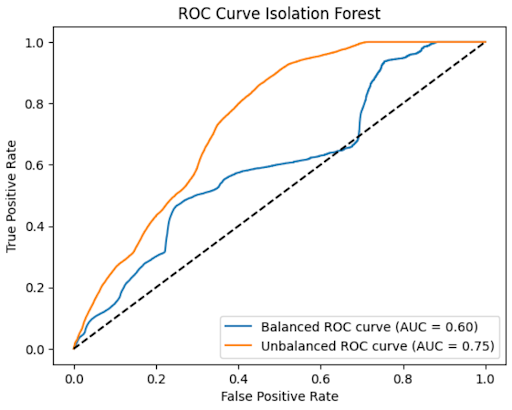
\includegraphics[width=\linewidth]{image/roc_isolation_forest.png} % Change to the path where your image is stored
\caption{ROC curves for Isolation Forest}
\label{fig:my_photo} % Label for referencing the figure in text
\end{figure}

Following these findings, we proceeded to train various models on the balanced version of Dataset 1. Table 2 demonstrates various performance metrics for the chosen models. 

\begin{table}[ht]
\centering

\label{tab:card_trans_metrics}
\begin{tabular}{lccccc}
\toprule
Model & Accuracy & Precision & F1 & Recall\\
\midrule
LR* & 0.93 & 0.92& 0.93& 0.95\\
Decision Tree & 0.99& 0.99& 0.99& 0.99\\
XGBoost & 0.99& 0.99& 0.99& 0.99\\
\bottomrule
\end{tabular}
\caption{Dataset 1 Evaluation Metrics  (*LR denotes Logistic Regression)}
\end{table}

\begin{figure}[htbp]
\centering
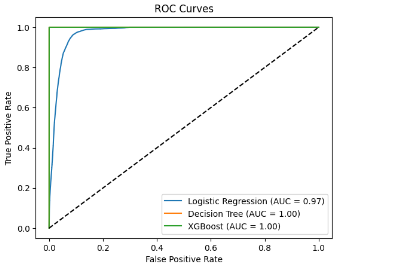
\includegraphics[width=\linewidth]{image/roc_other_models.png} % Change to the path where your image is stored
\caption{ROC curves for other models}
\label{fig:my_photo} % Label for referencing the figure in text
\end{figure}

Results from all other chosen models (Decision Tree, Logistic Regression, XGBoost) demonstrated excellent classification performance across many metrics, including accuracy, precision, F1 score, recall, and AUC. Skeptical of these ideal results, we sought to infer different feature interactions and importances through the usage of the Logistic Regression model's coefficients. Using the coefficients, we could interpret how each feature impacts the log-odds of a classification being legitimate or fraudelent. Regression coefficients for each feature are outlined in Table 3. 

\begin{table}[ht]
\centering

\label{tab:features}
\begin{tabular}{lc}
\toprule
Feature & Coefficient \\
\midrule
distance\_from\_home & 1.89 \\
distance\_from\_last\_transaction & 1.78 \\
ratio\_to\_median\_purchase\_price & 2.99\\
repeat\_retailer & -0.97\\
used\_chip & -0.73\\
used\_pin\_number & -4.38\\
online\_order & 3.49\\
\bottomrule
\end{tabular}
\caption{Features and Regression Coefficients}
\end{table}

Intuitively inferring these coefficients, we were able to make the following observations: 

\begin{itemize}
  \item Holding all else constant, for every unit increase in \texttt{ratio\_to\_median\_purchase\_price} we expect an increase of \textbf{2.99} in likelihood that the purchase was \textbf{fraudulent}.
  \item Holding all else constant, when the purchase was made with a \texttt{repeat\_retailer} we expect an increase of \textbf{0.97} in likelihood that the purchase was \textbf{legitimate}.
  \item Holding all else constant, when the purchase was made with a \texttt{used\_pin\_number} we expect an increase of \textbf{4.38} in likelihood that the purchase was \textbf{legitimate}.
  \item Holding all else constant, when the purchase was made with a \texttt{online\_order} we expect an increase of \textbf{3.34} in likelihood that the purchase was \textbf{fraudulent}.
\end{itemize}

\subsection{Dataset 2}

Accounting for the results using the balanced version of Dataset 1, we proceeded straightway using the balanced version of Dataset 2 on Decision Tree, Logistic Regression, and XGBoost models. Performance metrics remained substantially high across all models despite using entirely new data (see Table 4 and Figure 3).

\begin{table}[ht]
\centering

\label{tab:card_trans_metrics}
\begin{tabular}{lccccc}
\toprule
Model & Accuracy & Precision & F1 & Recall\\
\midrule
LR & 0.96 & 0.98 & 0.96 & 0.95\\
Decision Tree & 0.99& 0.99& 0.99& 0.99\\
XGBoost & 0.99& 0.99& 0.99& 1.0\\
\bottomrule
\end{tabular}
\caption{Dataset 2 Evaluation Metrics}
\end{table}


\begin{figure}[htbp]
\centering
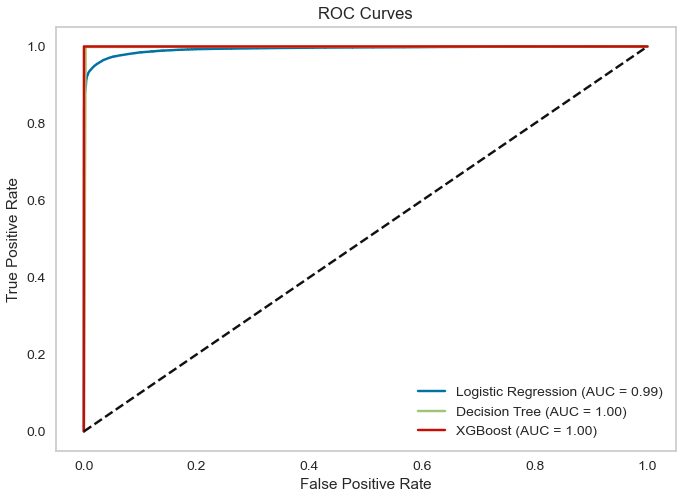
\includegraphics[width=\linewidth]{image/anon_roc_other_models.png} % Change to the path where your image is stored
\caption{ROC curves for other models}
\label{fig:my_photo} % Label for referencing the figure in text
\end{figure}


Evaluating feature importance among the principal components in these results, we decided to use the XGBoost 'Gain' metric which is given by the following formula:

\[
\text{Gain} = \frac{1}{2} \left[ \frac{G_L^2}{H_L + \lambda} + \frac{G_R^2}{H_R + \lambda} - \frac{(G_L + G_R)^2}{H_L + H_R + \lambda} \right] - \gamma
\]
\\

Essentially, each term within the brackets represent the score of splitting on a node, or how well the node acheives a reduction in loss, minus the regularization parameter. We found that one particular feature significantly maximized 'Gain' over all other features, 
which was \texttt{V14} (see Figure 4).


\begin{figure}[htbp]
\centering
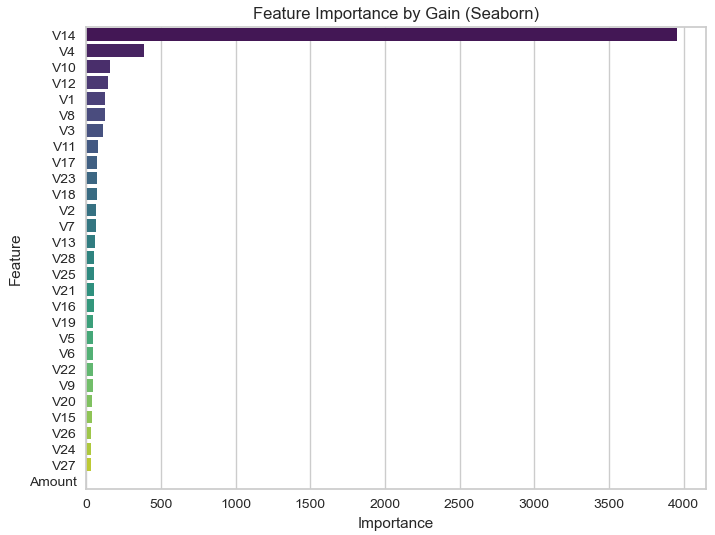
\includegraphics[width=\linewidth]{image/v14_gain_graph.png} % Change to the path where your image is stored
\caption{Feature importance by Gain in Dataset 2}
\label{fig:my_photo} % Label for referencing the figure in text
\end{figure}


\section{Data Improvements and New Results}

The exceptional results we obtained through nearly all methods in both datasets was unprecedented and instigated a pivot from seeking to improve performance metrics. We instead directed our efforts towards optimization through feature engineering and feature space adjustments. We hypothesized that with a simplification of our given feature space, computational efficiency would be increased, and model generalizability would theoretically improve. 

\subsection {Dataset 1 Feature Engineering}

Abstracting the interpretable meanings of the orignal features in Dataset 1, 3 new features were created, as shown in Table 5. 

\begin{table}[ht]
\centering

\label{tab:features}
\begin{tabular}{lc}
\toprule
Feature & Data Type \\
\midrule
price\_online & continuous \\
chip\_and\_pin & boolean \\
total\_distance & continuous \\
\bottomrule
\end{tabular}
\caption{New features for Dataset 1}
\end{table}

\texttt{price\_online} is derived through multiplying features \texttt{ratio\_to\_median\_purchase\_price} and \texttt{online\_order}. The intuition behind this combination places emphasis on abnormally high or low purchases when made online. 
\texttt{chip\_and\_pin} is calculated by the negative product of the two boolean features \texttt{used\_chip} and \texttt{used\_pin\_number}. Essentially, if a chip and pin are used within a transaction, this feature provides more weight to the probability a transaction is legitimate.
\texttt{ total\_distance} is measured by taking the sums of the individual logarithmic values of \texttt{distance\_from\_home} and \texttt{distance\_from\_last\_transaction}. We speculated that if a distance is within a threshold of a distance away from home or another origin, that feature weight should remain relatively consistent. For instance, if a purchase is made 100 miles away, another purchase made 500 miles away shouldn't increase the probability the transaction is fraud by a direct factor of 5. 

The base features from which these new features were calculated were dropped from the dataset. Performance metrics were then evaluated on previous models (see Table 6). We noted that, despite a retention in performance across metrics of accuracy, precision. F1 score, and recall, scores were marginally deducted by roughly \text{3\%}. Further, we compared a confusion matrix of our predictions from our transformed data to our previous data (see Figures 5, 6).

\begin{table}[ht]
\centering

\label{tab:card_trans_metrics}
\begin{tabular}{lccccc}
\toprule
Model & Accuracy & Precision & F1 & Recall\\
\midrule
LR & 0.91 & 0.91 & 0.91 & 0.91\\
Decision Tree & 0.94& 0.95& 0.94& 0.95\\
XGBoost & 0.96& 0.94& 0.96& 0.98\\
\bottomrule
\end{tabular}
\caption{Transformed Dataset 1 Evaluation Metrics}
\end{table}

\begin{figure}[htbp]
\centering
\includegraphics[width=\linewidth]{image/og\_confusion\_matrix} % Change to the path where your image is stored
\caption{Confusion Matrix for original Dataset 1}
\label{fig:my_photo} % Label for referencing the figure in text
\end{figure}

\begin{figure}[h]
\centering
\includegraphics[width=\linewidth]{image/new\_confusion\_matrix} % Change to the path where your image is stored
\caption{Confusion Matrix for transformed Dataset 1}
\label{fig:my_photo} % Label for referencing the figure in text
\end{figure}


As seen by comparing the two confusion matrices, the number of false negatives nearly doubled after we made these modifications to Dataset 1. We believe this is likely attributed to one or more of our engineered features losing original information that better discretized between certain transactions that were fraudelent. 

\subsection{Dataset 2 Feature Reduction}

After analyzing feature importances through 'Gain' as explored earlier, we decided to drop all features except the top 5 ranked in importance by 'Gain', which were features \texttt{V14, V4, V10, V12, V1}. After running previous models on the new feature space, we received the following results contained in Table 7. 

\begin{table}[ht]
\centering

\label{tab:card_trans_metrics}
\begin{tabular}{lccccc}
\toprule
Model & Accuracy & Precision & F1 & Recall\\
\midrule
LR & 0.95 & 0.95 & 0.95 & 0.93\\
Decision Tree & 0.99 & 0.99 & 0.99 & 0.99\\
XGBoost & 0.98& 0.99& 0.99& 0.99\\
\bottomrule
\end{tabular}
\caption{Transformed Dataset 2 Evaluation Metrics}
\end{table}

As evidenced by the our results, reducing the dimension of the original feature space from 28 principal components to 5 preserved nearly the totality of our models' predictive ability. Though the exact meanings behind these important 5 features is only known to the owners of the original dataset, we can clearly see that they effectively capture critical aspects of the patterns between fraudulent and legitimate credit card activity.





\section{Conclusion and Discussion}

What are our best results? How does they compare against expectations? What could be improved? 

\section{Future Considerations}

How does our work apply to real world scenarios? Additional options + hypothesises?


%% The file named.bst is a bibliography style file for BibTeX 0.99c
\bibliographystyle{named}
\bibliography{ijcai09}

\end{document}

